The overall methodology is to use a WiFi antenna to collect probe requests,
assign a unique identification based on the device that created the request,
aggregate them based on the unique identification for a specific time interval
to create an estimate of number of people at the location.
In this section we look at the characteristics of probe requests in detail,
outline the methodology used to collect these probe requests, 
look at the uncertainities and biases in the process and 
device methods to overcome these issues.

\subsection{Probe Requests}
Probe request is a low level packet sent by a mobile device as a means of
"scanning" for various access points available at a specific location.
This packet consists information about the mobile device including but not 
limited to,
Media Access Control address - A two part 12 bit identifier where the first part
identifies the manufacturer of the device and the second part identifies the
device itself. This MAC address is of two types, global - the real identifier
of the device which doesnt change and local - virtual, random addresses used
for temporary situations.
Sequence number of the packet to keep track of the replies.
The access points for which the packet is being sent to.
Capabilities of the device.
We can also infer other things about the packet such as
time at which the packet has been received,
total length of the packet
time it took to transmit the packet
Signal strength of the packet.
All of this can help us identifying the packets and label them when they are transmitted by the same device.

\subsection{Data Collection}
The manual count was undertaken using an Android application on a mobile phone: the researcher touched the phone’s screen every time an individual pedestrian footfall was counted, and this was recorded as a time-stamp.
An initial analysis revealed that the fields - SSID and tags - were very sparse and did not provide much information for our cleaning process.
In addition, the duration field was closely related to the length of the probe request and provides no new information.
Therefore, we removed these fields from further analysis.
We eliminated the noise from devices outside the area of interest by removing all the probe requests which reported a "low" signal strength.
This classification of "high" vs "low" was performed using a k-means classification algorithm.
The cut-off point for the collected data was -71 dBm.
\subsection{Removing uncertainties}
\subsubsection{Signal Strength}
\lipsum[1-3]
\subsubsection{Device Fingerprinting}
We then used the fields - OUI, lengths and sequence number - to tackle the noise from devices which anonymised the probe requests.
OUI and length were used to split the dataset into groups of probe requests from similar devices, and each subset was classified further using a graph based clustering algorithm where each cluster corresponded to a unique device.
The algorithm created a graph where the probe requests represented the nodes, and links are created between them based on the following rules: 
	\begin{enumerate}
		\item A link could go only forward in time. 
		\item A link could exist between nodes with a maximum time difference of $\alpha$ (time threshold).
		\item A link could go from low to high sequence numbers.
		\item A link could exist between nodes with a maximum sequence number difference of $\beta$ (sequence threshold).
		\item A node could have only one incoming link and one outgoing link, which is the shortest of all such possible links.
	\end{enumerate}
The nodes were then classified based on the unique connected component they belonged to.
This classification was assigned as the unique identifier for the anonymised probe requests.

\begin{figure} \begin{center}
	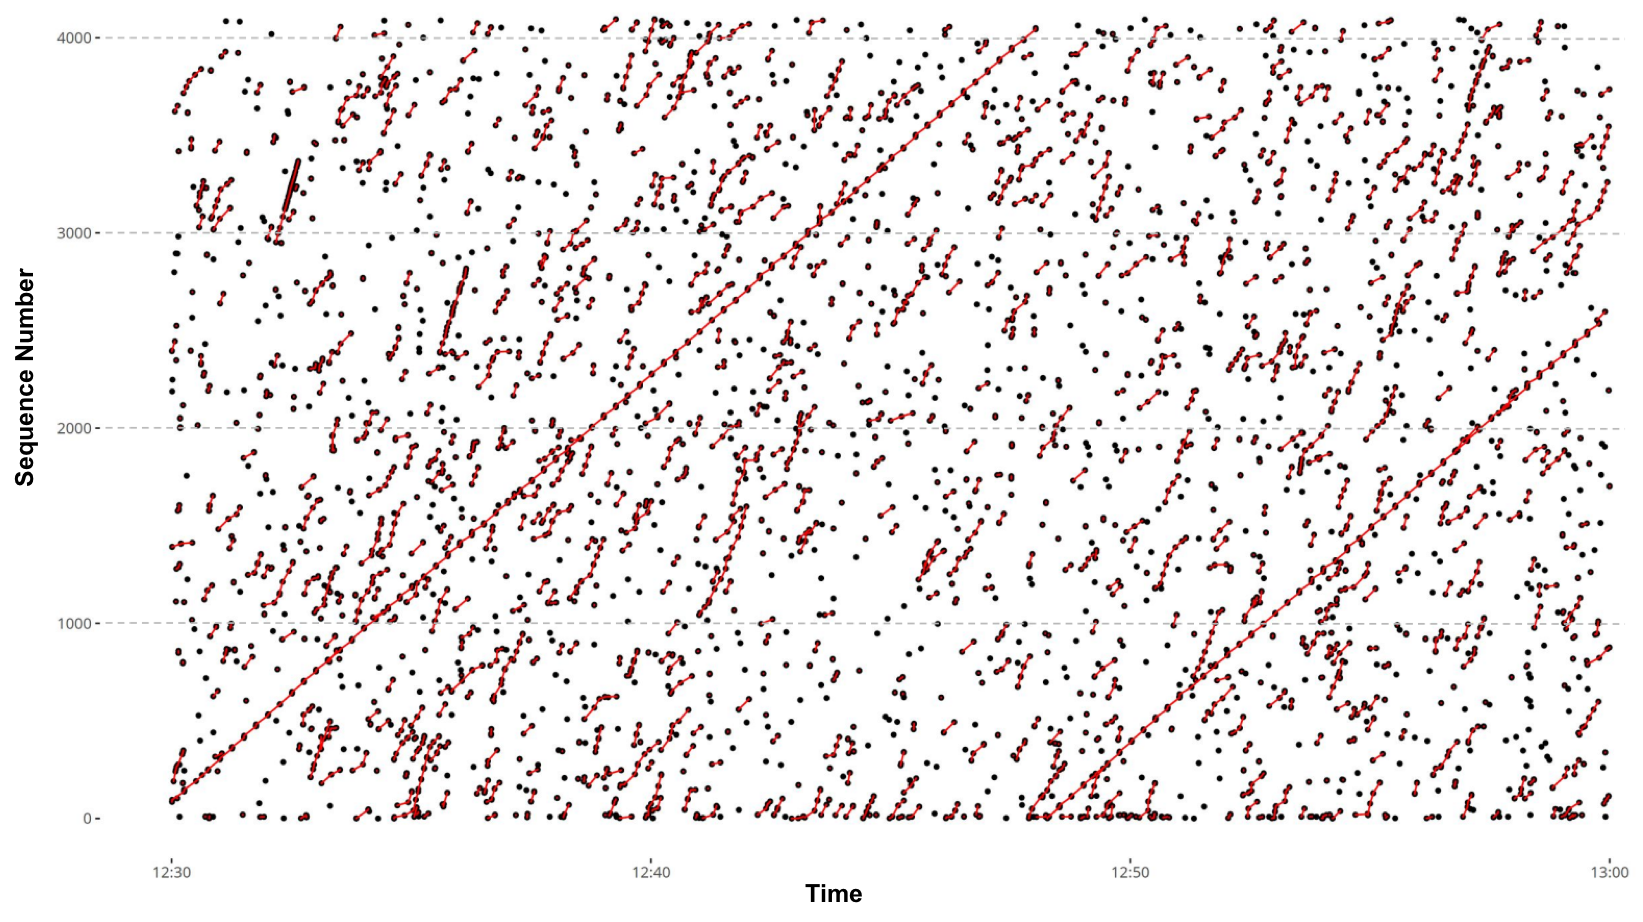
\includegraphics [width=\linewidth,trim=4 4 4 4,clip] {images/methodology_clustering.png}
	\caption{Clustering probe requests based on increasing sequence numbers present in them.}
	\label{clustering_pilot}
\end{center} \end{figure}

\subsubsection{Calibration}
\lipsum[1-2]
